\documentclass[12pt, a4paper]{report}

% Packages :

\usepackage[french]{babel}
\usepackage[utf8]{inputenc}
\usepackage[T1]{fontenc}
\usepackage[pdftex, pdfauthor={Bacomathiques}]{hyperref}
\usepackage{sectsty}
\usepackage[explicit]{titlesec}
\usepackage{xcolor}
\usepackage{amsmath}
\usepackage{amssymb}
\usepackage{amsthm}
\usepackage{fourier}
\usepackage{titlesec}
\usepackage{fancyhdr}
\usepackage{catchfilebetweentags}
\usepackage[french, capitalise, noabbrev]{cleveref}
\usepackage[fit, breakall]{truncate}
\usepackage[margin=3cm]{geometry}
\usepackage{tocloft}
\usepackage{tikz}
\usepackage{tocloft}
\usepackage{microtype}
\usepackage{listings}
\usepackage{tabularx}
\usepackage{calc}
\usepackage[export]{adjustbox}
\usepackage[most]{tcolorbox}
\usepackage{standalone}
\usepackage{xlop}
\usepackage{etoolbox}
\usepackage{environ}

\usetikzlibrary{arrows.meta}
\usetikzlibrary{trees}

% Paramètres :

\author{Bacomathiques}
\definecolor{graphe}{HTML}{93c9ff}
\setcounter{MaxMatrixCols}{12}
\setlength{\parindent}{0pt}
\setlength{\fboxsep}{0pt}
%\pdfsuppresswarningpagegroup=1

% Code :

\lstdefinestyle{style}{
	backgroundcolor=\color{white},
	commentstyle=\em\color[HTML]{999988},
	keywordstyle=\bfseries,
	identifierstyle=\normalfont,
	stringstyle=\color[rgb]{0.87, 0.07, 0.27},
	basicstyle=\ttfamily\color{black},
	breakatwhitespace=false,
	breaklines=true,
	captionpos=b,
	keepspaces=true,
	numbers=left,
	numbersep=5pt,
	showspaces=false,
	showstringspaces=false,
	showtabs=false,
	tabsize=2,
	numbers=none
}

\lstset{style=style}
\lstset{
	literate=
	{á}{{\'a}}1
	{à}{{\`a}}1
	{ã}{{\~a}}1
	{é}{{\'e}}1
	{ê}{{\^e}}1
	{í}{{\'i}}1
	{ó}{{\'o}}1
	{õ}{{\~o}}1
	{ú}{{\'u}}1
	{ü}{{\"u}}1
	{ç}{{\c{c}}}1
}

\lstset{
	framextopmargin=10pt,
	framexrightmargin=10pt,
	framexbottommargin=10pt,
	framexleftmargin=10pt,
	xleftmargin=10pt,
	xrightmargin=10pt,
}

% Couleurs :

\definecolor{title}{HTML}{912c21}
\definecolor{section}{HTML}{1c567d}
\definecolor{subsection}{HTML}{2980b9}

\definecolor{rule}{HTML}{c4c4c4}

\definecolor{formula}{HTML}{ebf3fb}
\definecolor{formula-left}{HTML}{3583d6}

\definecolor{tip}{HTML}{dcf3d8}
\definecolor{tip-left}{HTML}{26a65b}

\definecolor{demonstration}{HTML}{fff8de}
\definecolor{demonstration-left}{HTML}{f1c40f}

\definecolor{exercise}{HTML}{e0f2f1}
\definecolor{exercise-left}{HTML}{009688}

\definecolor{correction}{HTML}{e0f7fa}
\definecolor{correction-left}{HTML}{00bcd4}

\definecolor{toc}{HTML}{fceae9}
\definecolor{toc-left}{HTML}{e74c3c}
\definecolor{toc-dark}{HTML}{87281f}

% Titres :

\renewcommand{\thesection}{\Roman{section} - }
\renewcommand{\thesubsection}{\arabic{subsection}. }

\newcommand{\sectionstyle}{\normalfont\LARGE\bfseries\color{section}}
\titleformat{\section}{\sectionstyle}{\thesection #1}{0pt}{}
\titleformat{name=\section, numberless}{\sectionstyle}{#1}{0pt}{}

\newcommand{\subsectionstyle}{\normalfont\Large\bfseries\color{subsection}}
\titleformat{\subsection}{\subsectionstyle}{\thesubsection #1}{0pt}{}
\titleformat{name=\subsection, numberless}{\subsectionstyle}{#1}{0pt}{}

\titlelabel{\thetitle\ }

% Table des matières :

\addto\captionsfrench{\renewcommand\contentsname{}}
\renewcommand{\cftsecpagefont}{\color{toc-dark}}
\renewcommand{\cftsubsecpagefont}{\color{toc-dark}}
\renewcommand{\cftsecleader}{\cftdotfill{\cftdotsep}}
\renewcommand{\cftsecfont}{\bfseries}
\renewcommand{\cftsecpagefont}{\bfseries\color{toc-dark}}
\setlength{\cftbeforetoctitleskip}{0pt}
\setlength{\cftaftertoctitleskip}{0pt}
\setlength{\cftsecindent}{0pt}
\setlength{\cftsubsecindent}{20pt}
\setlength{\cftsubsecnumwidth}{20pt}

% Commandes :

\newcommand{\newpar}{\\[\medskipamount]}
\newcommand{\lesson}[3]{%
	\newcommand{\level}{#1}%
	\newcommand{\id}{#2}%
	\hypersetup{pdftitle={#3}}
	\begin{center}%
		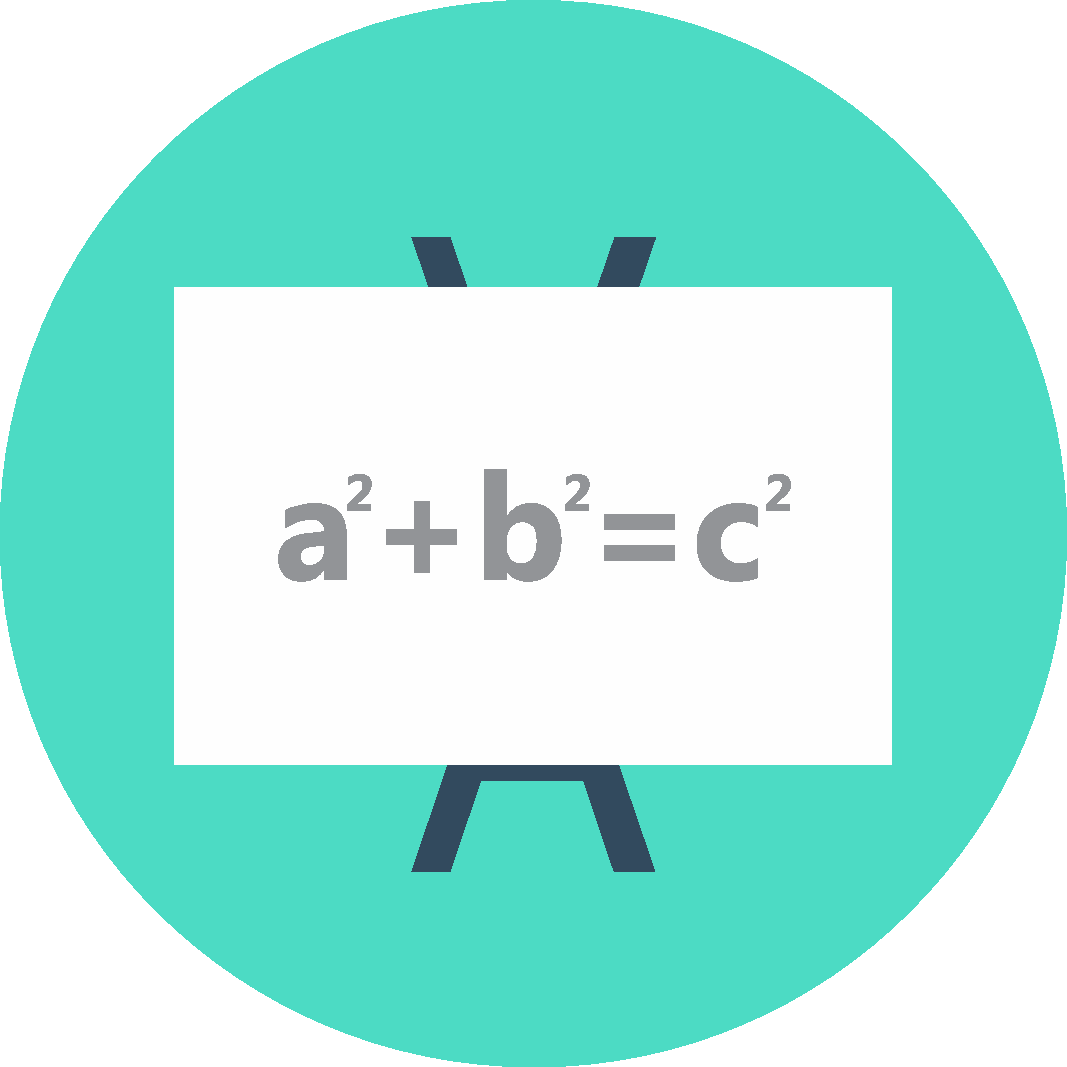
\includegraphics[width=150px]{\imagespath/bacomathiques}%
		
		\vspace{30pt}%
		{\Huge\color{title} #3}%
		
		\vspace{10pt}%
		{Bacomathiques --- \href{https://bacomathiqu.es/cours/#1/#2}{\color{section} https://bacomathiqu.es}}%
		
		\vspace{20pt}%
	\end{center}%
	\begin{toc}
		\tableofcontents%
	\end{toc}
	\thispagestyle{empty}%
	\newpage%
	\setcounter{page}{1}%
}
\newcommand{\imagespath}{../../images}
\newcommand{\lessonimagespath}{\imagespath/lessons/\level/\id/}
\newcommand{\includelatexpicture}[2][\textwidth - 100pt]{%
	\begin{center}%
		\resizebox{#1}{!}{%
			\input{\lessonimagespath#2}%
		}%
	\end{center}%
	\medskip%
}
\newcommand{\includeimage}[1]{%
	\begin{center}%
		\includegraphics{\lessonimagespath#1}%
	\end{center}%
	\medskip%
}
\newcommand{\includerepresentation}[1]{%
	\begin{center}%
		\setlength{\fboxrule}{0.5pt}%
		\href{https://www.geogebra.org/m/#1}{\includegraphics[width=\textwidth-1pt,fbox]{\lessonimagespath#1}}%
	\end{center}%
}
\newcommand{\floor}[1]{\lfloor #1 \rfloor}

\makeatletter
\newcommand\inputcontent{\@ifstar{\inputcontent@star}{\inputcontent@nostar}}
\newcommand{\inputcontent@star}[1]{%
	\ExecuteMetaData[#1]{content}%
}
\newcommand{\inputcontent@nostar}[1]{%
	\newpage%
	\inputcontent@star{#1}%
}
\makeatother

\let\oldsection\section
\renewcommand\section{\clearpage\oldsection}
\newcommand{\contentwidth}[1][medium]{}

% En-têtes :

\pagestyle{fancy}

\renewcommand{\sectionmark}[1]{\markboth{\thesection \ #1}{}}

\fancyhead[R]{\truncate{0.23\textwidth}{\color{title}\thepage}}
\fancyhead[L]{\truncate{0.73\textwidth}{\color{title}\leftmark}}
\fancyfoot[C]{\scriptsize \href{https://bacomathiqu.es/cours/\level/\id}{\texttt{bacomathiqu.es}}}

\makeatletter
\patchcmd{\f@nch@head}{\rlap}{\color{rule}\rlap}{}{}
\patchcmd{\headrule}{\hrule}{\color{rule}\hrule}{}{}
\makeatother

% Environnements :

\newenvironment{nosummary}{}{}
\newcommand{\tcolorboxtitle}[2]{\setlength{\fboxsep}{2.5pt}\hspace{-10pt}\colorbox{#1-left}{\hspace{8pt}\MakeUppercase{#2} \hspace{2pt} \includegraphics[height=0.8em]{\imagespath/bubbles/#1}\hspace{5pt}}}
\newcommand{\tcolorboxsubtitle}[2]{\ifstrempty{#2}{}{\textcolor{#1-left}{\large#2}\\[\medskipamount]}}
\tcbset{
	frame hidden,
	boxrule=0pt,
	boxsep=0pt,
	enlarge bottom by=8.5pt,
	enhanced jigsaw,
	boxed title style={sharp corners,boxrule=0pt,coltitle={white},titlerule=0pt},
	fonttitle=\fontsize{6pt}{6pt}\bfseries\boldmath,
	top=10pt,
	right=10pt,
	bottom=10pt,
	left=10pt,
	arc=0pt,
	outer arc=0pt,
}
\newtcolorbox{toc}[1][]{
	colback=toc,
	borderline west={3pt}{0pt}{toc-left},
	title=\tcolorboxtitle{toc}{Table des matières},
	colbacktitle=toc,
	before upper={\tcolorboxsubtitle{toc}{#1}}
}
\newtcolorbox{formula}[1][]{
	colback=formula,
	borderline west={3pt}{0pt}{formula-left},
	title=\tcolorboxtitle{formula}{À retenir},
	colbacktitle=formula,
	before upper={\tcolorboxsubtitle{formula}{#1}}
}
\newtcolorbox{tip}[1][]{
	colback=tip,
	borderline west={3pt}{0pt}{tip-left},
	title=\tcolorboxtitle{tip}{À lire},
	colbacktitle=tip,
	before upper={\tcolorboxsubtitle{tip}{#1}}
}
\newtcolorbox{demonstration}[1][]{
	colback=demonstration,
	borderline west={3pt}{0pt}{demonstration-left},
	title=\tcolorboxtitle{demonstration}{Démonstration},
	colbacktitle=demonstration,
	before upper={\tcolorboxsubtitle{demonstration}{#1}}
}

\NewEnviron{whitetabularx}[1]{%
	\renewcommand{\arraystretch}{2.5}
	\colorbox{white}{%
		\begin{tabularx}{\textwidth}{#1}%
			\BODY%
		\end{tabularx}%
	}%
}

% Longueurs :

\newlength{\espacetitreliste}
\setlength{\espacetitreliste}{-16pt}
\newcommand{\entretitreetliste}{\vspace{\espacetitreliste}}

\begin{document}
	%<*content>
	\lesson{terminale}{12}{algorithmique}{Algorithmique}

	\header{caption}{On retrouve les algorithmes en informatique mais également en robotique.}

	\header{excerpt}{L'algorithmique est l'étude et la production de règles et techniques qui
		sont impliquées dans la définition et la conception d'algorithmes, c'est-à-dire
		de processus systématiques de résolution d'un problème permettant de décrire précisément
		des étapes pour résoudre un problème algorithmique. \newpar Ce cours qui n'est pas au
		programme va quand même vous servir sur les exercices contenant des algorithmes
		au baccalauréat.}

	\header{difficulty}{5}

	\section{Définition}

	\textbf{Un algorithme} est une suite finie et ordonnée d’opérations ou d'instructions permettant de résoudre un problème ou d'obtenir un résultat. Ainsi, faire une recette de cuisine ou encore effectuer une division euclidienne à la main sont des exemples d'algorithmes.
	\newpar
	Dans ce cours, nous travaillerons à la fois avec des algorithmes \href{https://python.org}{Python} et des algorithmes en pseudo-code.

	\section{Instructions}

	\subsection{Création de variables}

	\textbf{Créer une variable} permet de réserver un espace pour y stocker des données quelconques.
	\newline
	On donne un nom à chaque espace pour le repérer : ce sont les noms de variables.
	Dans certains langages, on leur donne également un type (entier, réel, ...) pour travailler avec (ce qui n'est pas le cas dans Python).

	\begin{formula}[En python]
		\entretitreetliste
\begin{lstlisting}[language=python]
nombre = 0 # On crée la variable "nombre" et on lui assigne la valeur 0.
chaine = 'Bonjour' # On crée la variable "chaine" et on lui assigne la valeur 'Bonjour'.
\end{lstlisting}
	\end{formula}

	\begin{tip}[Exemple (tiré du sujet de Pondichéry 2017)]
		\includeimage{algorithme-1.png}
		Ici nous avons quatre variables : $R$ et $S$ qui sont des réels et $n$ et $k$ qui sont des entiers.
	\end{tip}

	\subsection{Affectations de valeurs}

	Comme dit précédemment, les variables sont des ``espaces'' dans lequel il est possible de stocker des informations.
	\newpar
	Cependant, après avoir créé cet espace, celui-ci est encore vide. C'est pourquoi on doit le ``remplir'' : c'est \textbf{l'affectation d'une valeur à une variable}.
	\newpar
	Il existe plusieurs manières d'affecter une valeur à une variable : soit on lui donne directement sa valeur dans l'algorithme, soit on demande à l'utilisateur d'entrer une valeur (il faut garder à l'esprit que nos algorithmes sont faits pour être utilisés par des utilisateurs).

	\begin{formula}[En python]
		\entretitreetliste
\begin{lstlisting}[language=python]
x = int(input('Veuillez entrer une valeur : ')) # L'utilisateur va entrer une valeur, on la convertir en entier et on va affecter celui-ci à notre variable "x".
y = 2*x + 10 # Une fois fait, "y" va prendre la valeur 2 * x + 10. Par exemple, si l'utilisateur entre "10", "y" vaudra 30.
\end{lstlisting}
	\end{formula}

	\begin{tip}[Exemple (tiré du sujet de Pondichéry 2017)]
		\includeimage{algorithme-1.png}
		Ici on donne à $S$ la valeur $0$, mais on demande à l'utilisateur d'entrer la valeur de la variable $n$ (l'utilisateur entrera un entier, car la variable $n$ ne peut contenir que des entiers).
	\end{tip}

	Une fois que l'on a affecté une valeur à une variable, il est encore possible de la changer !

	Les \textbf{listes} sont des types de variables particuliers. Ce sont en effet, ``des variables qui contiennent des variables''.

	\begin{formula}[En python]
		\entretitreetliste
\begin{lstlisting}[language=python]
fruits = ['pomme', 'banane', 'poire']
fruits.append('cerise') # On peut ajouter un objet à notre liste.
del fruits[0] # On peut également supprimer un objet de la liste en fonction de son index (ici, on supprime le premier).
fruits.remove('pomme') # Mais on peut aussi en supprimer un avec sa valeur.
# Beaucoup d'autres opérations sur les listes sont disponibles (longueur, renversement, ...). N'hésitez pas à vous renseigner !
\end{lstlisting}
	\end{formula}

	\subsection{Affichage de variables}

	Nos algorithmes étant faits pour être utilisés, il faut donc \textbf{retourner un résultat} sinon ceux-ci seraient inutiles. C'est pourquoi, on peut ``afficher'' les valeurs des variables (les montrer à l'utilisateur).

	\begin{formula}[En python]
		\entretitreetliste
\begin{lstlisting}[language=python]
print('Voici la valeur de "maVariable" :', maVariable) # Permet d'afficher la valeur de "maVariable".
\end{lstlisting}
	\end{formula}

	\begin{tip}[Exemple (tiré du sujet de Métropole 2017)]
		\includeimage{algorithme-2.png}
		Une fois l'algorithme terminé, on affiche la valeur de la variable $N$ (on remarque que $N$ a pris plusieurs valeurs différentes au cours de l'algorithme mais qu'on affiche uniquement la valeur finale de la variable).
	\end{tip}

	\section{Blocs d'instructions}

	\subsection{Définition}

	Les blocs d'instructions sont des parties de l'algorithme (ce sont des ``algorithmes dans l'algorithme'') qui s'exécutent suivant certaines conditions propres aux différents blocs d'instructions.

	\subsection{Les blocs SI et SINON}

	Les blocs \textbf{SI} et \textbf{SINON} sont des blocs d'instructions très utilisés qui permettent de tester une condition : si elle est réalisée, on va exécuter les instructions se situant sous le bloc SI et sinon, on va exécuter celles se situant sous le bloc SINON.

	\begin{formula}[En python]
		\entretitreetliste
\begin{lstlisting}[language=python]
x = 2 # On attribue à "x" la valeur 2.
if x == 3: # Si "x" est égal à 3...
	print('"x" est égal à 3.') # ... Alors on affiche ce message. Mais ici, "x" vaut 2 donc ce message ne sera jamais affiché.
else: # Sinon...
	print('"x" n\'est pas égal à 3.') # ... On affiche ce message.
\end{lstlisting}
	\end{formula}

	\begin{tip}[Exemple (test de parité)]
		\includeimage{algorithme-3.png}
		Si la partie entière de $\frac{N}{2}$ est égale à $\frac{N}{2}$ (ce n'est vrai que pour les entiers pairs), alors on donne à $R$ la valeur 0. Sinon on lui donne la valeur 1.
		\newline
		En fin d'algorithme, on affiche la valeur de $R$ : soit 0 si $N$ est pair, soit 1 si $N$ est impair.
	\end{tip}

	\subsection{La boucle POUR}

	La \textbf{boucle POUR} est un bloc d'instruction qui s'exécute et qui va faire prendre à une variable toutes les valeurs comprises dans un ensemble d'entiers.

	\begin{formula}[En python]
		\entretitreetliste
\begin{lstlisting}[language=python]
for i in range(-5, 6): # Pour chaque entier entre -5 (inclus) et 6 (exclu)...
	print(i) # ... On affiche cet entier.
\end{lstlisting}
	\end{formula}

	\begin{tip}[Exemple (calcul des termes d'une suite)]
		\includeimage{algorithme-4.png}
		Cet algorithme permet de calculer les termes d'une suite $(u_n)_{n \in \mathbb{N}}$ définie par récurrence :
		\newpar
		$\begin{cases} u_0 = 1\\ u_{n+1} = u_n + \frac{1}{n}\end{cases}$ pour $n$ entier.
		\newpar
		On demande à l'utilisateur d'entrer une variable $N$, et pour $n$ variant de 1 jusqu'à $N$ ($n$ prendra tour à tour les valeurs 1, 2, 3, ..., $N-1$, $N$), on va calculer les termes de la suite.
	\end{tip}

	\subsection{La boucle TANT QUE}

	Cette boucle, différente de la boucle POUR, permet d'exécuter son bloc d'instructions tant qu'une certaine condition est valable.

	\begin{formula}[En python]
		\entretitreetliste
\begin{lstlisting}[language=python]
x = 100 # On affecte à "x" la valeur 100.
while x > 10: # Tant que x est supérieur à 10...
	x = x / 2 # On divise x par 2 (i.e. on affecte à "x" la valeur x/2).
	print(x) # On affiche la valeur de "x".
\end{lstlisting}
	\end{formula}

	\begin{tip}[Exemple (tiré du sujet de Métropole 2017)]
		\includeimage{algorithme-2.png}
		Ici, tant que $N - \ln(N^2 + 1)$ est inférieur à $A$, on affecte une nouvelle valeur à la variable $N$.
	\end{tip}

	\begin{nosummary}
		\section{Algorithmes sur l'ordinateur}

		Il est possible de tester et de vous entraîner aux algorithmes sur votre ordinateur, voire directement sur votre smartphone !

		\begin{tip}[Quelques logiciels d'algorithmique]
			Divers logiciels à télécharger, dont certains ne nécessitant pas d'installation sont disponibles :
			\begin{itemize}
				\item \href{https://python.org}{Python}
				\item \href{https://www.algogo.xyz}{Algogo}
				\item \href{http://www.xm1math.net/algobox/}{AlgoBox}
				\item \href{https://scratch.mit.edu/}{Scratch}
				\item \href{http://proglab.fr/}{Proglab}
			\end{itemize}
		\end{tip}
	\end{nosummary}
	%</content>
\end{document}
